%%%%%%%%%%%%%%%%%%%%%%%%%%%%%%%%%%%%%%%%%%%%%%%%%%%%%%%%%%%%%%%%%%%%%%%%%%%%%%%%
%2345678901234567890123456789012345678901234567890123456789012345678901234567890
%        1         2         3         4         5         6         7         8

\documentclass[letterpaper, 10 pt, conference]{ieeeconf}  % Comment this line out if you need a4paper

%\documentclass[a4paper, 10pt, conference]{ieeeconf}      % Use this line for a4 paper

\IEEEoverridecommandlockouts                              % This command is only needed if 
                                                          % you want to use the \thanks command

\overrideIEEEmargins                                      % Needed to meet printer requirements.

% See the \addtolength command later in the file to balance the column lengths
% on the last page of the documet

% The following packages can be found on http:\\www.ctan.org
\usepackage{graphicx} % for pdf, bitmapped graphics files
%\usepackage{epsfig} % for postscript graphics files
%\usepackage{mathptmx} % assumes new font selection scheme installed
%\usepackage{times} % assumes new font selection scheme installed
\usepackage{amsmath} % assumes amsmath package installed
%\usepackage{amssymb}  % assumes amsmath package installed

%\usepackage{subcaption}
%\usepackage{adjustbox}

\title{\LARGE \bf
Adaptive Estimator as Task Monitor for Telerobotic Servicing Missions
}


\author{Xiao Li and Peter Kazanzides% <-this % stops a space
%\thanks{$^{1}$Albert Author is with Faculty of Electrical Engineering, Mathematics and Computer Science,
 %       University of Twente, 7500 AE Enschede, The Netherlands
  %      {\tt\small albert.author@papercept.net}}%
%\thanks{$^{2}$Bernard D. Researcheris with the Department of Electrical Engineering, Wright State University,
  %      Dayton, OH 45435, USA
    %    {\tt\small b.d.researcher@ieee.org}}%
}


\begin{document}


\maketitle
\thispagestyle{empty}
\pagestyle{empty}


%%%%%%%%%%%%%%%%%%%%%%%%%%%%%%%%%%%%%%%%%%%%%%%%%%%%%%%%%%%%%%%%%%%%%%%%%%%%%%%%
\begin{abstract}

This paper presents an online adaptive estimation system used for failure detection in telerobotic satellite servicing tasks. The system utilizes a recursive least squares estimator with vector-like forgetting factors, and have also included a throttling mechanism to ensure that the estimator is used only when the operation condition and input signals allow for reasonable outcomes. We have found that this throttling process is crucial in obtaining a steady estimator performance. Experiments are conducted on a da Vinci/WAM teleoperation system and results show that the proposed estimation system is relatively reliable in detecting various kinds of failures.

\end{abstract}

\begin{figure}[htbp]
\begin{center}
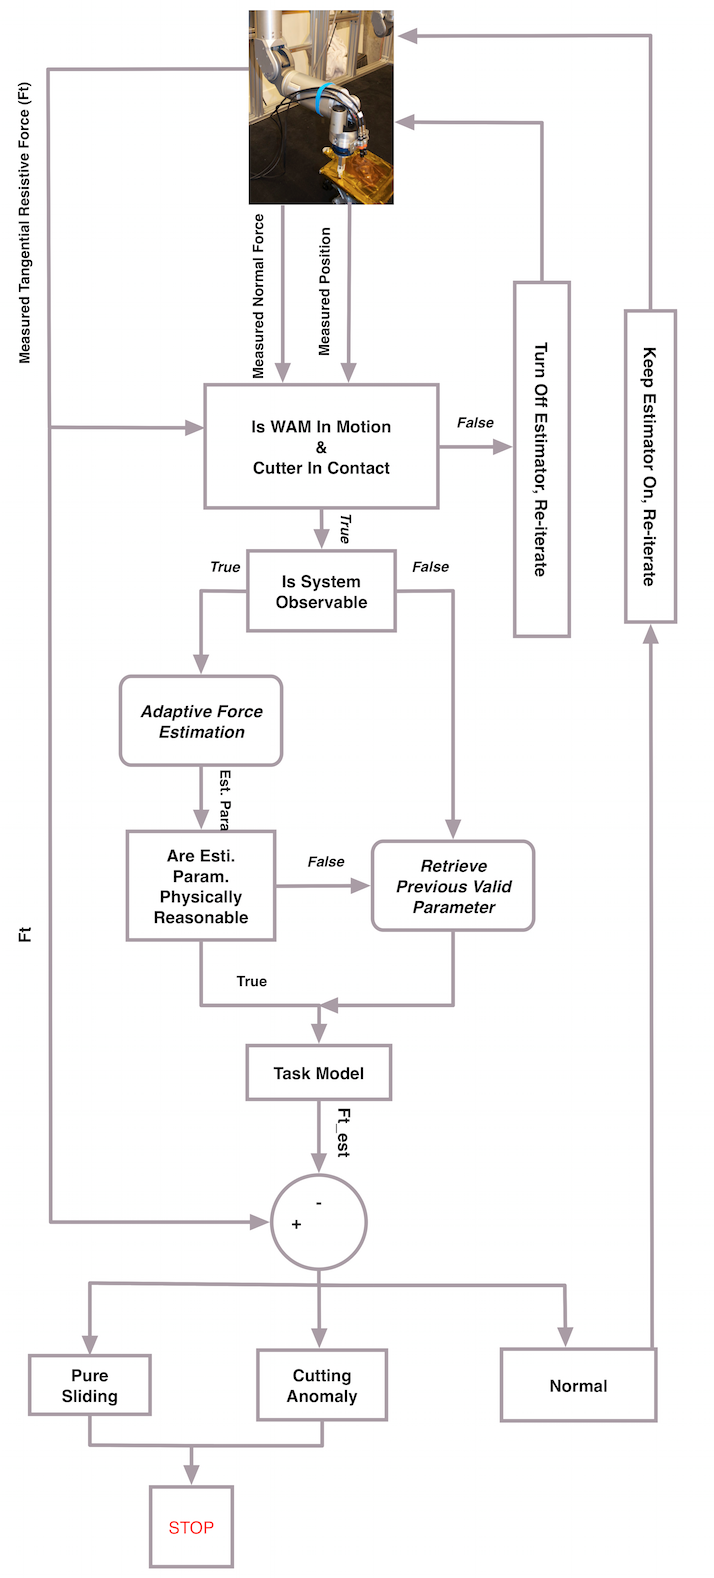
\includegraphics[width=0.45\textwidth]{figures/flowchart.png}
\caption{Estimator Schematic}
\label{fig:1}
\end{center}
\end{figure}

%%%%%%%%%%%%%%%%%%%%%%%%%%%%%%%%%%%%%%%%%%%%%%%%%%%%%%%%%%%%%%%%%%%%%%%%%%%%%%%%
\section{INTRODUCTION}
\label{sec:1}

For most teleoperated satellite servicing tasks, delay in the video feedback is in the order of seconds. This delay makes it difficult for the operator to stop the operation when unexpected events occur before any damage takes place. In this paper we consider the task of telerobotically cutting the tape that fastens the multi-layler insulation patch over the satellite access panel as part of the Robotic Satellite Refuelling Mission. Possible failure modes include bunching, tearing of the tape, the cutter moves off-course to regions where no task is defined as well as cutter jamming into hard surfaces or wires. To ensure that the remote manipulator identifies cutting failures promptly and pauses the operation before damage is done to the hardware, a task monitor loop is to be implemented on the remote side that assists the operator in detection of cutting anomalies. Such a task monitor takes the form of a state estimator that takes in task model parameters and produces a reasonable prediction of the force encountered by the cutter under normal cutting conditions and compare the prediction with the actual force measured by a force sensor mounted on the cutter. The expectation is that when a cutting anomaly occur the measured force will undergo rapid change and a difference in the estimated and measured values that exceeds a threshold will indicate the occurrence of a cutting failure. The experimental platform consists of a da Vinci master console and a Barrett WAM(Whole Arm Manipulator), and details of the experiment setup and procedure can be found in \cite{isha},\cite{2012iros},\cite{icra2013}.

Previous efforts have been made to accurately estimate interaction forces at the cutting interface. Most of the interaction force modelling techniques are developed under the context of machine operations (turning, milling, etc). However due to the fact that cutting and shearing processes with metal on metal contact are relatively uniform both at the interface as well as material properties, modelling usually assumes constant geometric and material parameters which is not the case here. In addition \cite{laparoscissors} ,\cite{scissors} have proposed methods to model the forces applied to scissors when cutting biological material. Both have considered the cutting process as a sequence of deformation and fracture phases and utilize energy-based fracture mechanics to aid modelling. \cite{analyScis} have studied modelling of scissors cutting force in general with a more geometric approach. \cite{needle} approached the problem of estimation of needle insertion force during surgical procedures with the help of a disturbance observer that estimate variations in friction force, and a recursive least square that turns this variation into changes in the friction parameters and hence obtain estimates of the force parameters. The estimation system proposed in this paper builds on \cite{isha} where the task model parameters are assumed constant. We have given consideration to the fact that material properties of the cutter and tape/MLI may vary (ageing, radiation, etc), the cutting process is unpredictable (cutter may penetrate the MLI and come into contact with other materials) and therefore a static estimator may not yield the most satisfactory results. Therefore we have proposed an adaptive estimation system with the aim that the estimator is able to conform to mild changes in the task model parameters but exposes an abnormal event by lagging behind a sudden change in measured force. 

The reminder of sections are structured as follows. Section \ref{sec:2} introduces the task model and the adaptive estimator. Section \ref{sec:3} provides the experimental setup, and the definition as well as values used for various tunable estimator parameters. Section \ref{sec:4} presents results followed by a detailed discussion of their significance. And section \ref{sec:5} concludes the article.
%\section{RELATED WORK}

%%%%%%%%%%%%%%%%%%%%%%%%%%%%%%%%%%%%%%%%%%%%%%%%%%%%%%%%%%%%%%%%%%
\section{FORCE MODEL AND ADAPTIVE ESTIMATOR}
\label{sec:2}
Since the cutting phase of interest disregards the initial step of inserting the cutter into the tape, the force model is taken to be a simple linear model given by 

\begin{equation}
F_t = \mu_k |F_n| + F_c
\label{eq:1}
\end{equation}


\noindent where $F_t$ is the total tangential force, $\mu_k$ is the kinetic coefficient of friction, $F_n$ is the contact normal force and $F_c$ is the cutting force due to shearing of the tape. Here we assume the positive $F_t$ and $F_c$ direction opposes the manipulator\rq{}s direction of motion (while cutting, $F_t$ is always greater than zero). The reason for choosing a simple model is that the cutting interface between the cutter and MLI is complex and unpredictable, to use a more complex model means that an estimator of higher dimension is required and the computational resources needed to execute the estimator online will be higher than desired. We feel that maintaining an acceptable failure detection accuracy while keeping the computational complexity at a minimum is important especially for space hardware that is limited in its computing abilities. As illustrated in \cite{isha}, there exists two cutting strategies (compression-based and tension-based) where the main difference is the sign of $F_n$,  an absolute value of $F_n$ is taken to ensure $\mu_k > 0$ at all times. \textit{The goal is to design an adaptive estimator such that for given measurements $\boldsymbol y = [F_t, F_n]^T$, parameters $\boldsymbol x = [\mu_k, F_c]^T$ can be recursively updated (denote the estimated parameters as $\hat{\boldsymbol x} = [\hat{\mu}_k, \hat{F}_k]^T$) and that $\hat{\boldsymbol x}$ adapt to mild changes in the cutting environment (material properties, cutter contact conditions, etc) but the resultant estimated tangential force given by $\hat{F}_t = \hat{\mu}_k F_n + \hat{F}_c $ distinguishes from the measured $F_t$ notably when a cutting abnormality happens}. The proposed approach utilizes a Recursive Least Squares (RLS) Estimator with vector-like forgetting. The choice of an RLS estimator is based on the fact that a the least squares estimator in its recursive form is least computation demanding, and since all historic information is preserved, with the help of vector-like forgetting factors the variational rate of individual parameters can be regulated thereby reinforcing the estimator with information of the physical world (such as for similar contact surface materials $\mu_k$ should be minimally varied but $F_c$ can change within a larger range). 


Equation \ref{eq:1} can be rewriten as 

\begin{equation}
F_t =  \begin{bmatrix} |F_n|  & 1 \end{bmatrix} \begin{bmatrix} \mu_k \\ F_c \end{bmatrix} := H^T\boldsymbol x
\label{eq:2}
\end{equation}

\noindent Let $P_k$ be the covariance of the estimated parameters, the adaptive estimation at step $k$ can be formulated as (according to \cite{forgetfactor})

\begin{equation}
K_k = P_{k-1}H_k(H_k^TP_{k-1}H_k + 1)^{-1}
\label{eq:3}
\end{equation}

\begin{equation}
\hat{\boldsymbol x}_k = \hat{\boldsymbol x}_{k-1}+K_k(\boldsymbol y_k - H_k^T\hat{\boldsymbol x}_{k-1})
\label{eq:4}
\end{equation}

\begin{equation}
P_k = \Lambda^{-1}(I - K_kH_k^T)P_{k-1}\Lambda^{-1}
\label{eq:5}
\end{equation}


\noindent where $\Lambda = diag(\lambda_1, \lambda_2, ..., \lambda_i)$ contains the forgetting factors for each parameter. The smaller $\lambda_i$ is, more weight is put on recent data  ($0<\lambda_i < 1$). By incorporating forgetting factors, the estimator can be controlled such that the kinetic coefficient of friction ($\mu_k$) is updated taking into account all historic data and the cutting force ($F_c$) updated putting more emphasis on recent data. This aligns with the physical truth that if the material properties of the cutter and MLI don\rq{}t change abruptly, $\mu_k$ should vary in a small range. But $F_c$ can vary drastically if cutting anomalies occur, this is also used to identify the occurrences of cutting failures (discussed in more detail in the following section). 
 
	In addition to forgetting factors, efforts have being made to identify situations where the estimator would give inaccurate results and proper throttling is employed to ensure  reasonable outcomes. The first of such situation is when the observability is low, which occurs when there is insufficient variations in the input vector $[F_n,1]^T$. To find a measure for variation, a \textit{Moving Window Least Squares} is imposed on the  measured normal force and a line $F_n=at+b$ is fitted through the data within each fixed size window. At time $t(n)$, the estimation goes by
	
\begin{equation}
\begin{bmatrix}
a \\ b
\end{bmatrix} = [\sum_{i=n-w}^{n}u(i)u(i)^T]^{-1}\sum_{i=n-w}^nu(i)F_n(i)
\end{equation}
	
\noindent Where $u(i)=[t(i),1]^T$ and $w$ is the window size. The slope of that line is used as a measure for  variation. A threshold is then set on $a$ and if $a(t) < threshold$ the adaptive estimator is turned off and failure identification is executed with the previous set of valid estimates. Through experiments we have also observed that due to various factors including noise, deformation of the cutting interface (and possibly other factors that have yet to be identified), some measurements yield negative $\hat{\mu}_c$ and/or $\hat{F_c}$ which is physically unreasonable and can affect the stability of later estimates. Therefore negative estimates are discarded and similar to what's mentioned above the previous valid estimates are used in a non-adaptive estimator which the resultant $\hat{F_t}$ is used for failure detection.  Figure~\ref{fig:1} illustrates the proposed estimator in its entire form.
 
%%%%%%%%%%%%%%%%%%%%%%%%%%%%%%%%%%%%%%%%%%%%%%%%%%%%%%%%%%%%%%%%%%%%%%%


%\section{EXPERIMENTAL RESULTS AND DISCUSSION} 
%\label{sec:3}
%This section establishes the experimental setup as well as the parameter values used in the the adaptive %estimator. Furthermore, the cutting anomalies that we aim to identify are also introduced. Results and %analysis are provided accordingly.

\section{EXPERIMENT AND ESTIMATOR SETUP}
\label{sec:3}

As is mentioned in section~\ref{sec:1} , the experimental system consists of a da Vinci master console and a Barrett WAM. Data from nine users have been collected each using the system to perform a number of trials with each trial defined as cutting through one vertical strip of tape as illustrated in figure~\ref{fig:2} below. Video, joint encoder and force sensor data are recorded for analysis.

\begin{figure}[htbp]
\begin{center}
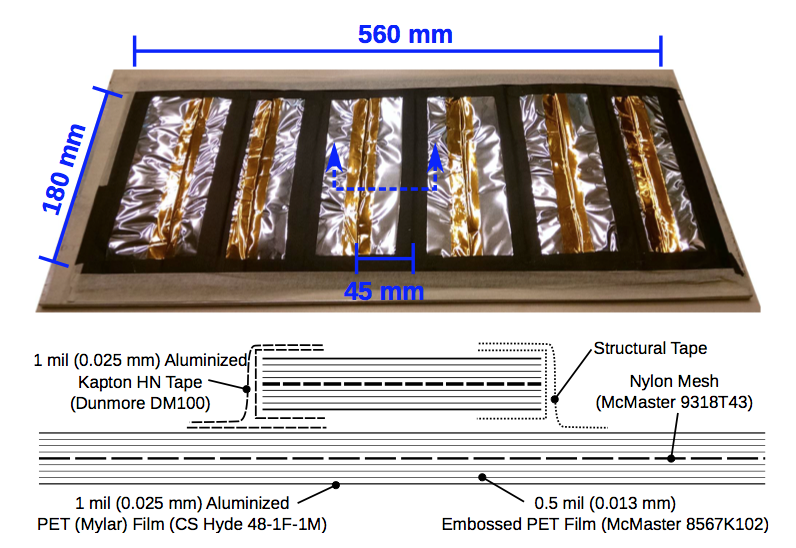
\includegraphics[width=0.45\textwidth]{figures/MLI.png}
\caption{Mock MLI Samples (image courtesy of Steve Vozar)}
\label{fig:2}
\end{center}
\end{figure}


The goal of the estimator is to accurately identify cutting anomalies. Here we have categorized cutting anomalies to two different most frequently occurring forms - cutter motion obstruction and MLI tearing. In addition the estimator is also designed to identify cutter slippage (sliding without cutting).  \noindent Figure~\ref{fig:3} below illustrates the cutting anomalies as they happen in the experiment.  


\begin{figure}[htbp]
\begin{center}
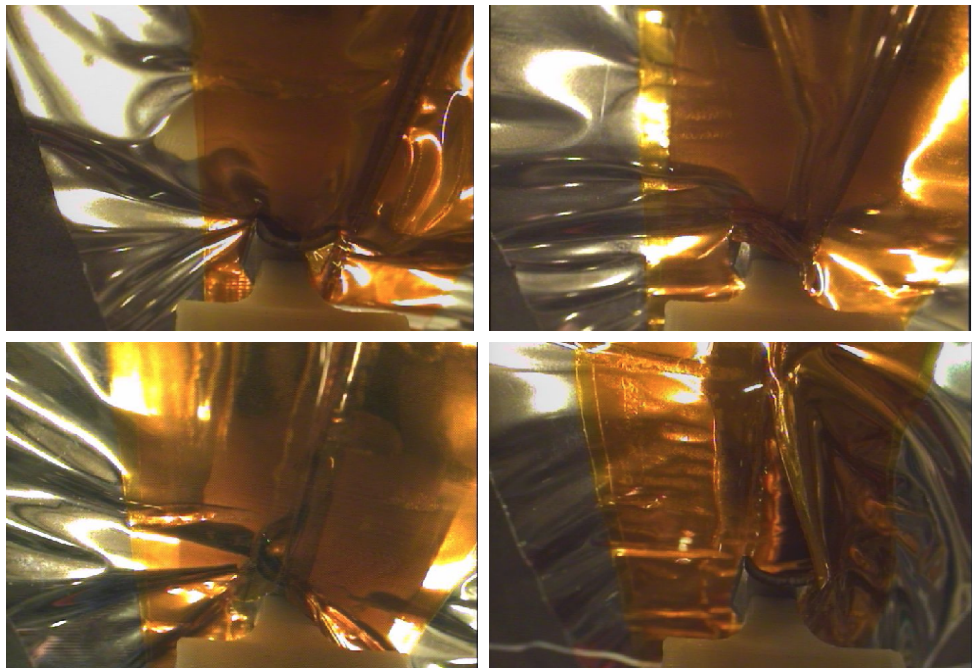
\includegraphics[width=0.45\textwidth]{figures/combine.png}
\caption{Illustration of cutting anomalies (top left) normal cutting condition, (top right) MLI bunching, (bottom left) cutter sinking into MLI, (bottom right) MLI tearing }
\label{fig:3}
\end{center}
\end{figure}

Table \ref{tab:1} below lists the estimator's evaluation criteria for cutting anomaly identification. Recalled that $F_t$  is the total resistive force measured by the force sensor, $F_n$ is the measured normal force (positive in compression and negative in tension), $\hat{F_t}$ is the estimated resistive force calculated from the estimated parameters.  Note also that since the evaluation criteria is the same for MLI/tape bunching and cutter sinking (\ref{fig:3} top right and bottom left), they are grouped into the same category as cutter motion obstruction.

\begin{table}[h]
\caption{Evaluation Criteria for Cutting Anomaly Identification}
\label{tab:1}
\begin{tabular}{|l|l|}
\hline
\multicolumn{1}{|l|}{} & \textbf{Evaluation Criteria} \\ \hline
\textbf{Cutter Motion Obstruction} & $F_t$  \textgreater $ \hat{F_t}$ + threshold \\ \hline
\textbf{MLI Tearing} & $F_n$ \textgreater 0 and $\hat{F_t}$ \textgreater $F_t$ + threshold \\ \hline
\textbf{Cutter Sliding Without Cutting} & $F_n$ \textless 0 and $\hat{F_t}$ \textgreater $F_t$ + threshold\\  \hline
\end{tabular}
\end{table}
 
We define a false positive to be an identification of failure when there isn't one and a false negative to be the opposite. As with the estimator, there exists a number of parameters that require presetting for proper performance and their values used for this experiment along with a brief explanation are tabulated in table~\ref{tab:2} below.


\begin{table}[h]
\caption{Estimator Parameter Values}
\label{tab:2}
\begin{tabular}{|c|c|c|}
\hline
\textbf{Est. Parameters} & \textbf{Value Used} & \textbf{Brief Description} \\ \hline
\begin{tabular}[c]{@{}c@{}}Obstruction\\threshold\end{tabular} & 1.8 (N) & \begin{tabular}[c]{@{}c@{}}For detection of cutter \\ motion obstruction\end{tabular} \\ \hline
\begin{tabular}[c]{@{}c@{}}Tearing\\threshold \end{tabular}& 1.8 (N) & \begin{tabular}[c]{@{}c@{}}For Detection of MLI \\ tearing\end{tabular} \\ \hline
\begin{tabular}[c]{@{}c@{}}Slippage\\threshold \end{tabular}& 1.8 (N) & \begin{tabular}[c]{@{}c@{}}For Detection of cutter sliding\\  without cutting\end{tabular} \\ \hline
\begin{tabular}[c]{@{}c@{}}Observability\\Threshold\end{tabular} & 0.35 & \begin{tabular}[c]{@{}c@{}} Threshold placed on slope \\of the line fitted through a section\\ of the  most recent input signal $F_n$ \\used to throttle the estimator at \\low observability level\end{tabular} \\ \hline
\begin{tabular}[c]{@{}c@{}}Window\\Size\end{tabular} & 80 & \begin{tabular}[c]{@{}c@{}}For the moving window \\least squares estimator used for \\observability identification\end{tabular} \\ \hline
\begin{tabular}[c]{@{}c@{}}Motion\\Threshold\end{tabular} & 0.001& \begin{tabular}[c]{@{}c@{}} Threshold on joint velocities \\used to identify if cutter is in motion \end{tabular} \\ \hline
\begin{tabular}[c]{@{}c@{}}$\lambda_{\mu_k}$ \end{tabular}& 0.99 & Forgetting factor for $\mu_k$ \\ \hline
\begin{tabular}[c]{@{}c@{}}$\lambda_{F_c}$\end{tabular} & 0.97 & Forgetting factor for $F_c$ \\ \hline
\end{tabular}
\end{table}

When failure occurs, the estimator is turned off and the previous valid estimate is again preserved for used when the cutting condition is normal again (which is another part of the throttling process ). This setup is likely to cause false positives due to high static friction at the start of each cutting motion, therefore the motion threshold is determined such that the estimator is turned on when the cutter has entered a steady cutting phase.


\section{RESULTS AND DISCUSSION}
\label{sec:4}
   
A total number of 22 experiment trials from 9 users are used to assess the performance of the estimator. A graphical interface is implement in ROS/Rviz as panel plugins (as shown in \ref{fig:4}) such that the user is able to monitor and interact with the estimator as he/she operates. In addition to the video streamed from cameras mounted on the cutter (bottom left), the interface provides real-time plots that shows (in order from top to bottom) the measured and estimated resistive force, the measured normal force, the difference between the measured and estimated which is used to indicate cutting anomaly, and lastly the variation in normal force that indicates the observability of the estimator. The dash lines in the third and fourth plot are visualizations of user-set thresholds to determine the occurrances of cutting anomalies. The value of these dash lines can be controlled with the slidebars on the upper right hand side of the interface. Incorporation of this feature gives the user a better idea of how the estimator is making decisions and helps with tuning of the estimator. In addition to the thresholds, the slidebar panel also includes tuning of more estimator parameters such as the forgetting factors, the window size for the normal force least square estimator, etc. The panel below the tuning slidebars shows in text the estimator's understanding of what the current cutting condition is, which includes four modes 'NORMAL', 'BUNCHING', 'TEARING' and 'SlIDING'. Since currently the system does not provide haptic feedback, the progress bars right above the video image provides the measurement readings of the normal and resistive force allowing the user conveniently monitor the forces imposed on the cutter while performing the cutting operation.      

\begin{figure}[htbp]
\begin{center}
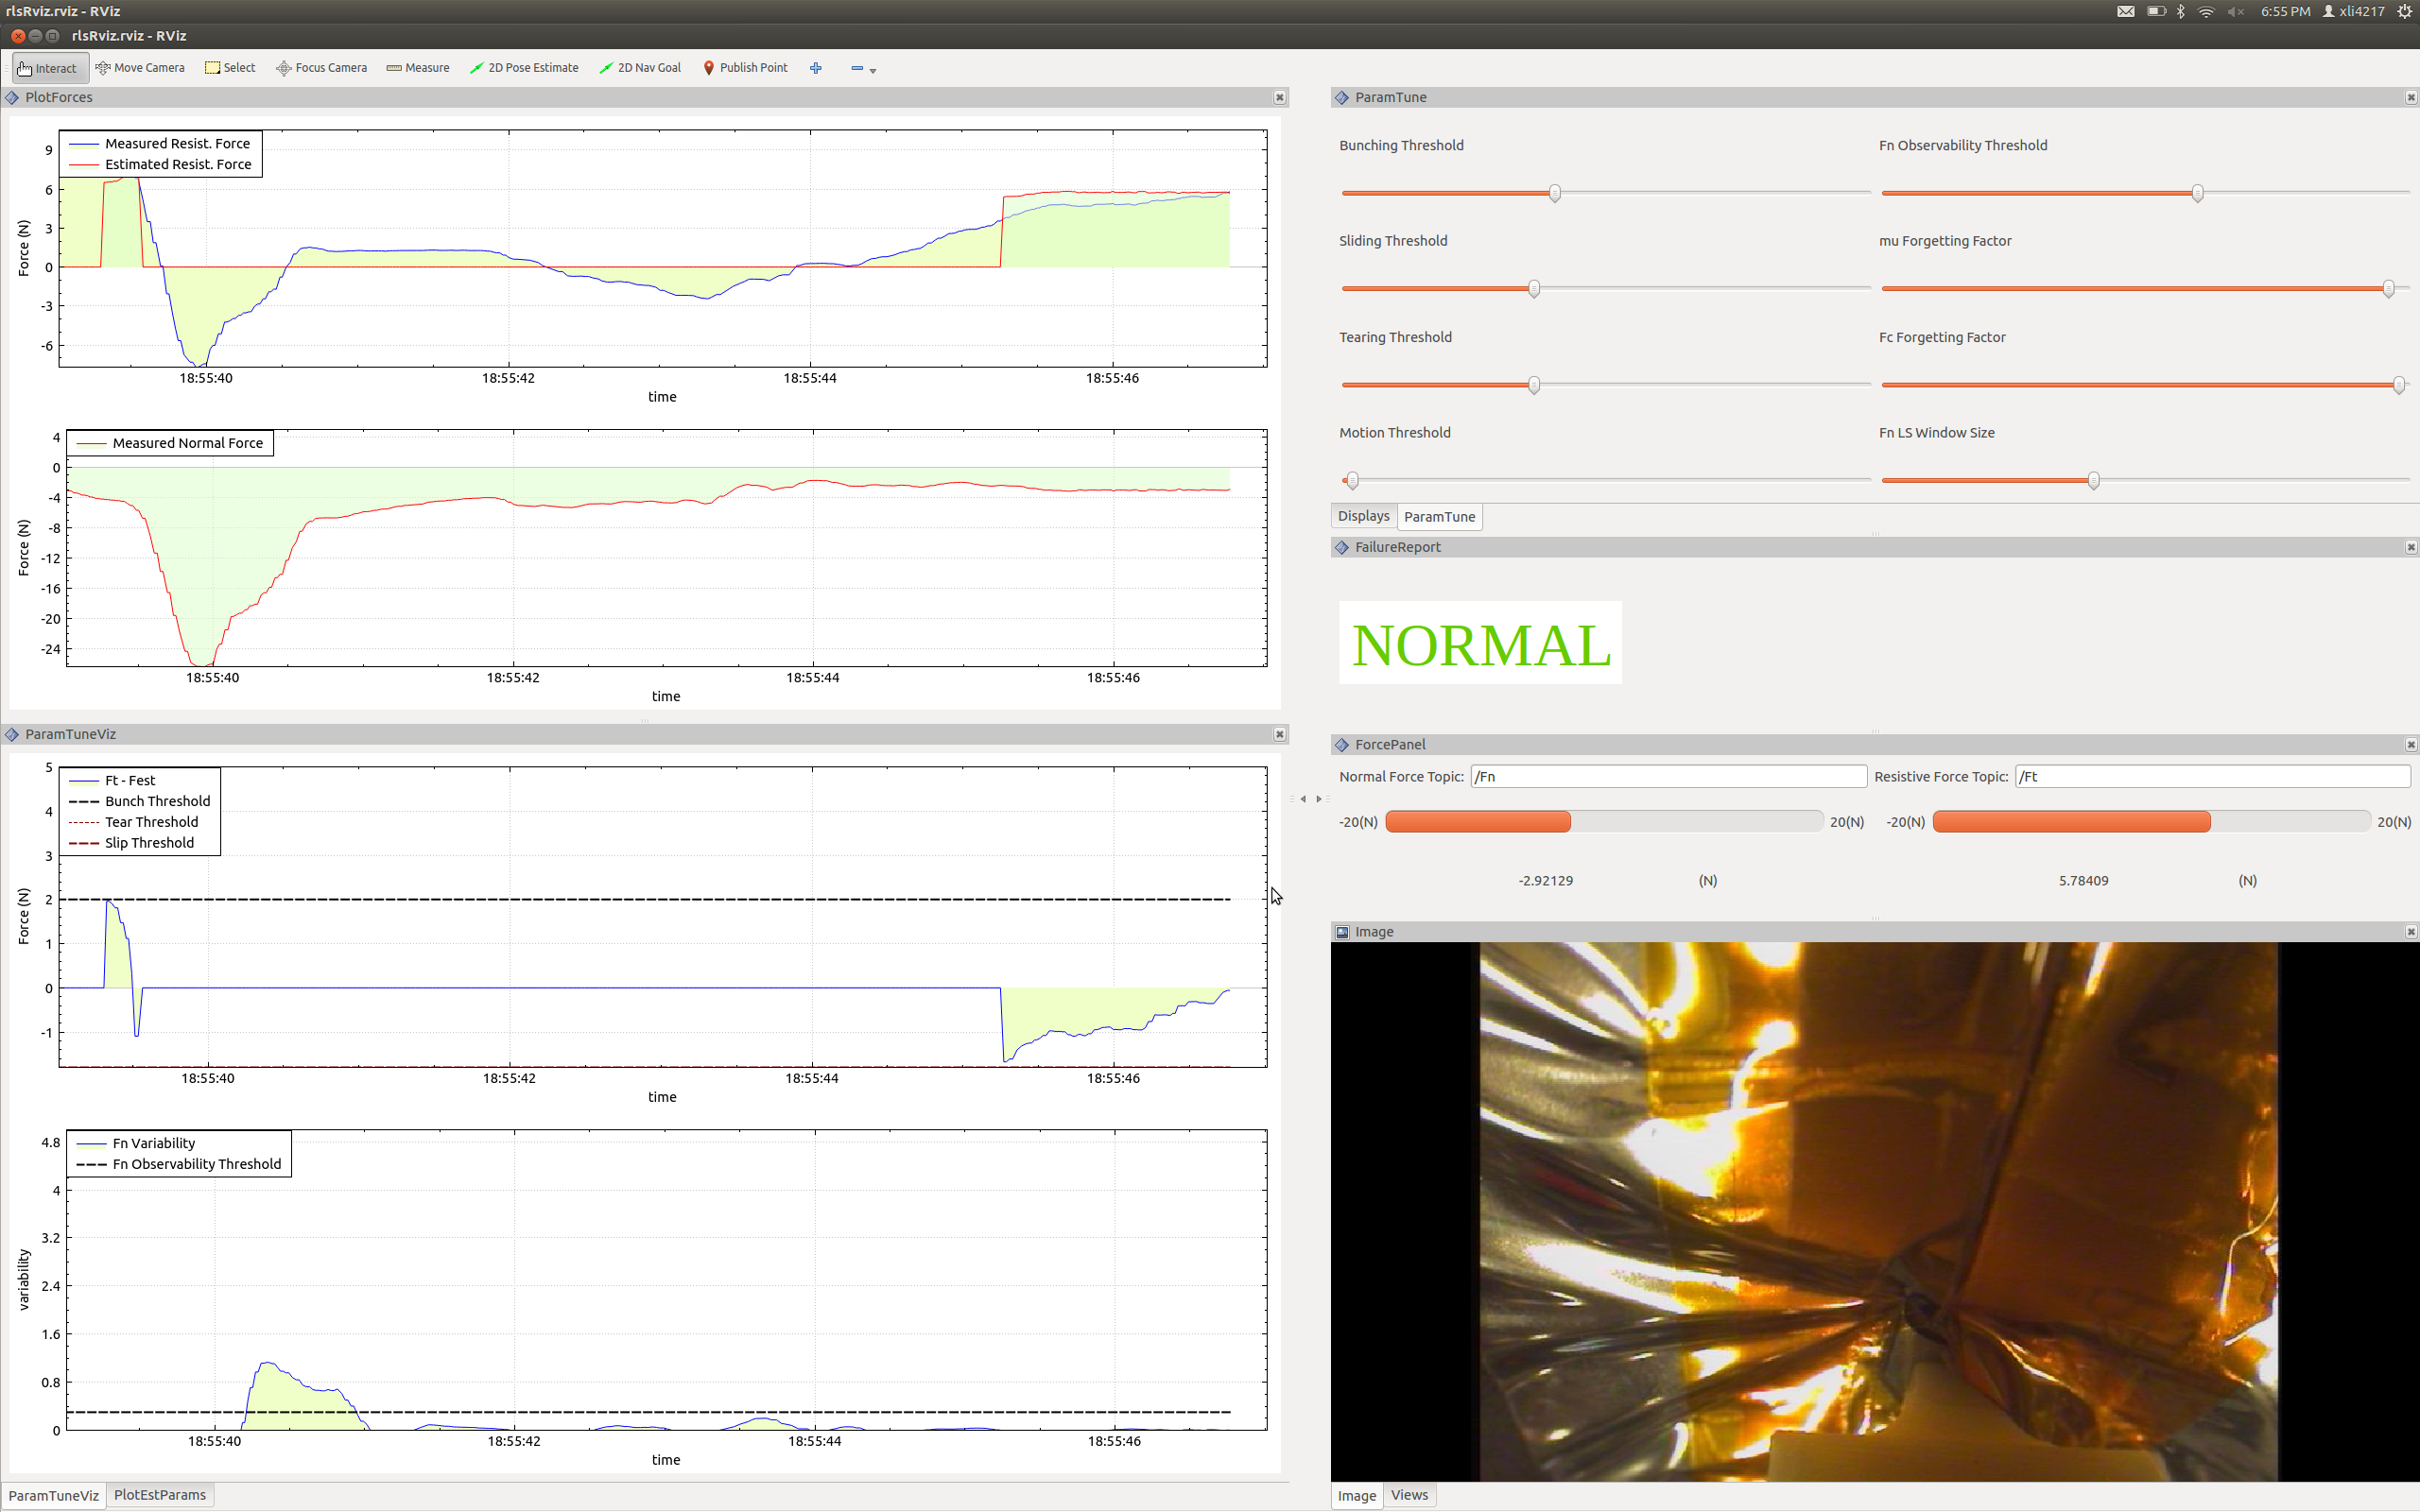
\includegraphics[width=0.5\textwidth]{figures/UI.png}
\caption{Estimator User Interface }
\label{fig:4}
\end{center}
\end{figure}
 
 Figure \ref{fig:5} below illustrates a sample outcome of the estimator. The first subplot shows the time series of the measured and estimated resistive force. The bars that intermittently goes to 10 are binary indicators of occurrences of cutting anomaly (which is also shown in the UI to inform the operator).  The pictures at the top are screenshots of the video stream when failures occur (in this case two occurrences of tearing). The estimator provides the estimated total resistive force, the kinetic coefficient of friction and cutting force. Looking at the figure,  there exists a clear strip-like texture to these estimated values. This is the result of estimator throttling under situations including cutter at rest, cutter not in contact, low observability of the system, unreasonable estimated values as well as occurrences of cutting anomalies (as mentioned above).  This throttling process ensures the estimated parameters to stabilize and be physically explainable. As a result, we can observe from the third and forth subplots that the estimated parameters started out with variations but gradually stabilizes over time indicating that under normal cutting conditions the kinetic coefficient of friction and cutting force is relatively constant. However situations such as  penetration of the cutter into the MLI and contact with adhesives can result in change of the parameter values and adaptation to these situations is the objective of the proposed estimator, and this can be reflected in the minor variations of the estimated values.


\begin{figure}[htbp]
\begin{center}
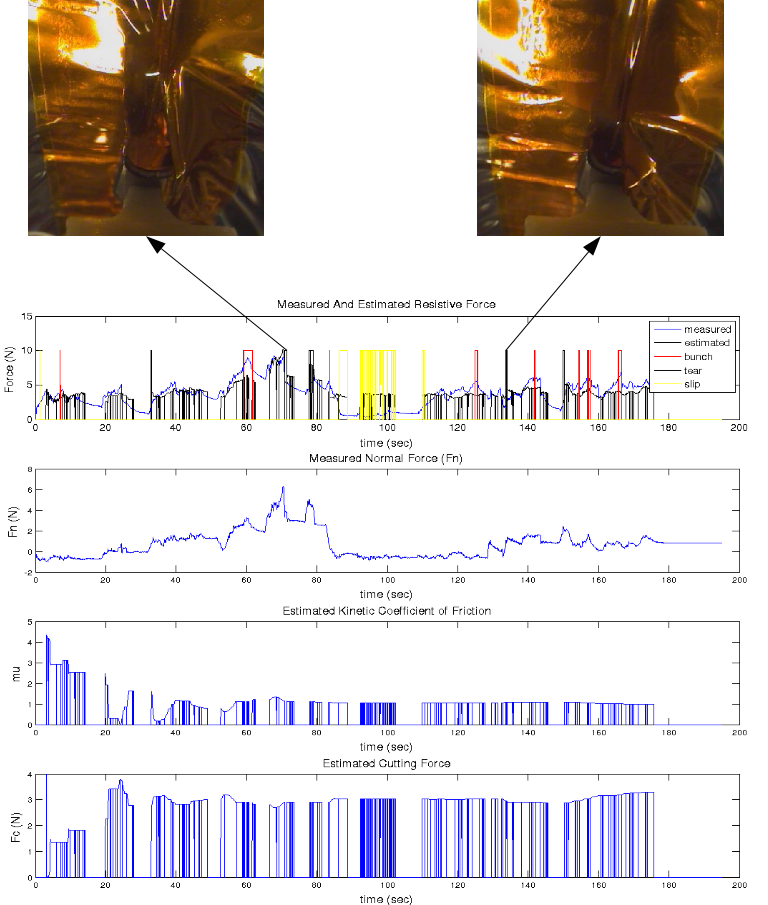
\includegraphics[width=0.47\textwidth]{figures/example.png}
\caption{Sample Estimator Output }
\label{fig:5}
\end{center}
\end{figure}

To further assess the effectiveness of this estimator, 22 set of experimental trials are conducted. Video data is recorded and analyzed to find occurrences of anomalies. The visually identified anomalies are then compared with that reported by the estimator and the result is listed in table \ref{tab:3}. 

\begin{table}[h]
\caption{Estimator Performance}
\label{tab:3}
\begin{tabular}{|c|c|c|c|}
\hline
 & \textbf{Visually Identified} & \textbf{False Positives} & \textbf{False Negatives} \\ \hline
\textbf{Bunching} & 56 & 5 & 2 \\ \hline
\textbf{Tearing} & 21 & 2 & 1 \\ \hline
\textbf{Slipping} & 22 & 3 & 1 \\ \hline
\multicolumn{2}{|c|}{\textbf{Total Clearly Observable Failures}} & \multicolumn{2}{c|}{17} \\ \hline
\multicolumn{2}{|c|}{\textbf{Total Identified}} & \multicolumn{2}{c|}{17} \\ \hline
\end{tabular}
\end{table}

\noindent Note that anomalies usually occur over a period of time, we say that the estimator has caught the anomaly if there is a reporting within this time or within three second prior to this visually identified failure period. Doing this takes into account the possibility that the failure may have started before there is a visual cue and when the visual cue shows the estimator may have already adapted to the measurements.  
Recall that a false positive is a failure reporting by the estimator when there isn't one visually identifiable and a false negative the opposite. As mentioned in the previous section, given consideration to the fact that static friction normally rises higher than kinetic friction, and when the cutter transitions from rest to motion the first set of parameters used in the task model are previous valid estimates (which includes the kinetic coefficient of friction $\mu_k < \mu_{static}$), the motion threshold is set to be a little higher than full sensitivity so that the estimator is turned on when cutter enters a steady cutting state to avoid false positive reporting each time the cutter starts to move and overcomes static friction. Have said the above, if the cutter is moving at a very low speed the estimator would simply be turned off and this accounts for the one bunching and one tearing false negative. In addition, detection of failure relies on a sudden change in the measured resistive force that results in a difference with the estimated resistive force due to the lag between the estimated parameter values and their real values. There is the possibility that the bunched tape/MLI accumulates gradually which gives the estimator enough time to adapt to this abnormal condition without reporting an anomaly. And this in fact is the case with the other bunching false negative. Because the tape and multi-layer insulation is deformable and relatively ductile, the cutting interface is highly unpredictable, relying on a single threshold to detect failure is a simplified but not the most accurate way. The false positives are results of this unpredictability. However there is also the possibility that failure may be happening underneath the surface and not visible by the video, for the time being we have considered this as a false positive but further investigation is necessary to obtain a more thorough assessment. It is important to note that out of all the anomalies identified, 17 are clearly visible and to different extents have jeopardized the cutting task and all are reported by the estimator. 

Out of the 22 trials recorded, the estimated parameters for 3 of the trials did not settle to a stabilized value and 2 have stabilized to values that we consider outliers. Discarding these 5 trials, the steady state estimates of the remaining 17 trials are plotted in figure \ref{fig:6}, \ref{fig:7}, \ref{fig:8} below. It can be observed that the steady state estimates between trials vary around a distinguishable mean. The prediction for steady state total resistive is calculated by $F_{t_{steady}}=\mu_{steady}\times4(N) + F_{c_{steady}}$ Specifically $\mu_{mean}=0.6, F_{c_{mean}}=3(N), F_{t_{steady}}=5.4(N)$. This to an extent proves that the estimator is able to perform consistently across trials.
 
\begin{figure}[htbp]
\begin{center}
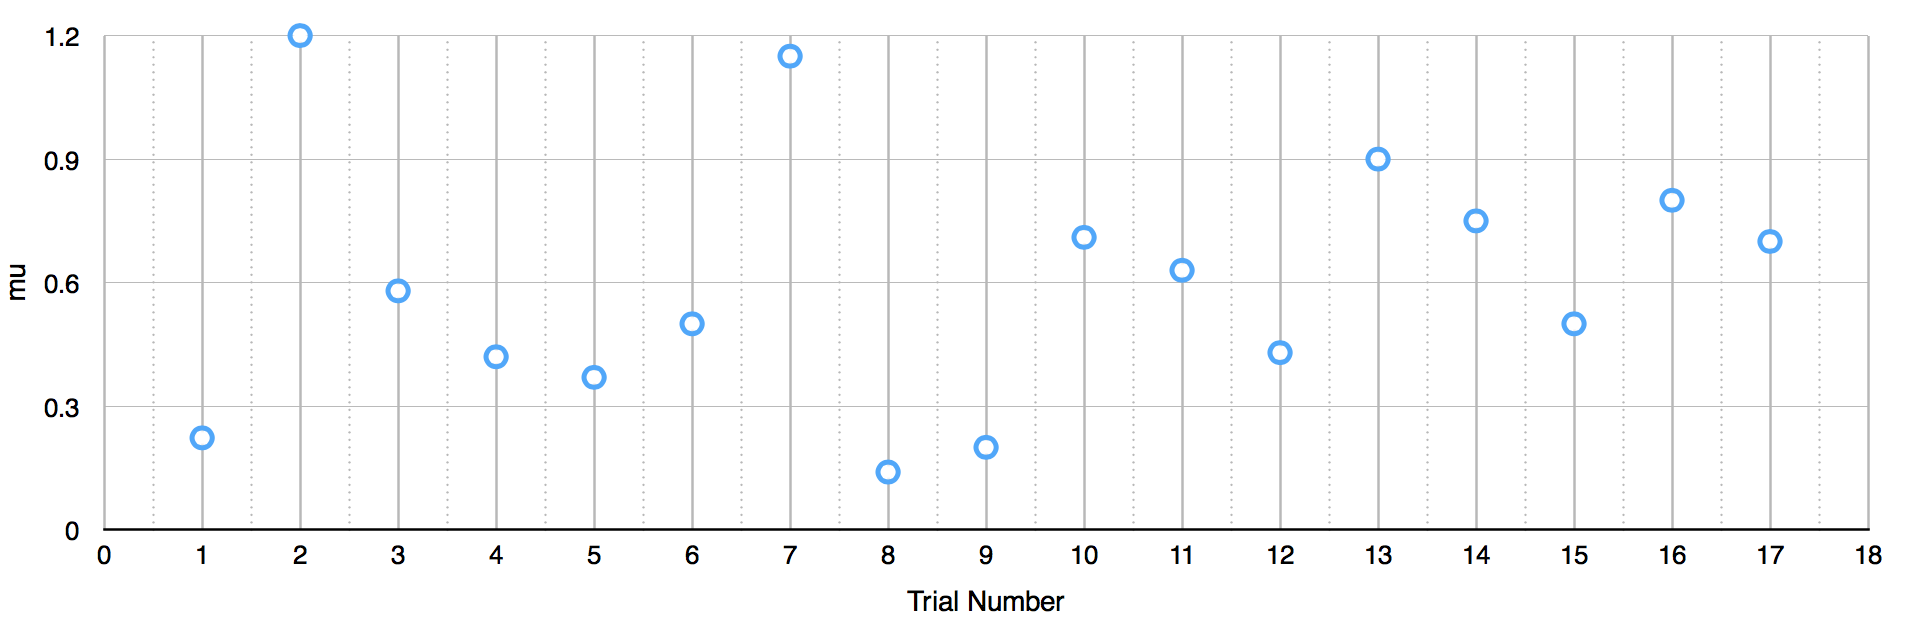
\includegraphics[width=0.5\textwidth]{figures/mu.png}
\caption{Steady State Estimated Coefficient of Kinetic Friction}
\label{fig:6}
\end{center}
\end{figure}

\begin{figure}[htbp]
\begin{center}
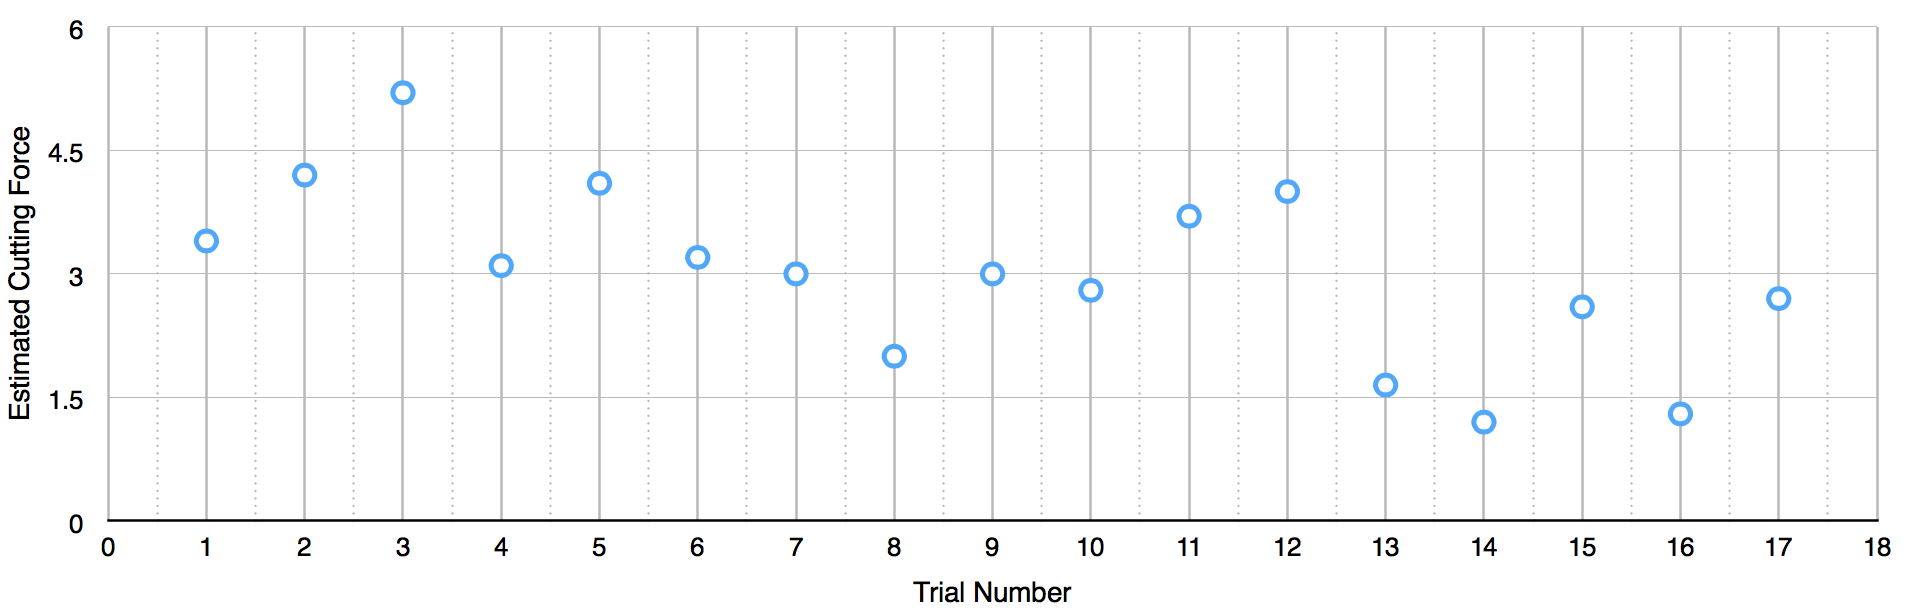
\includegraphics[width=0.5\textwidth]{figures/cuttingF.png}
\caption{Steady State Estimated Cutting Force}
\label{fig:7}
\end{center}
\end{figure}

\begin{figure}[htbp]
\begin{center}
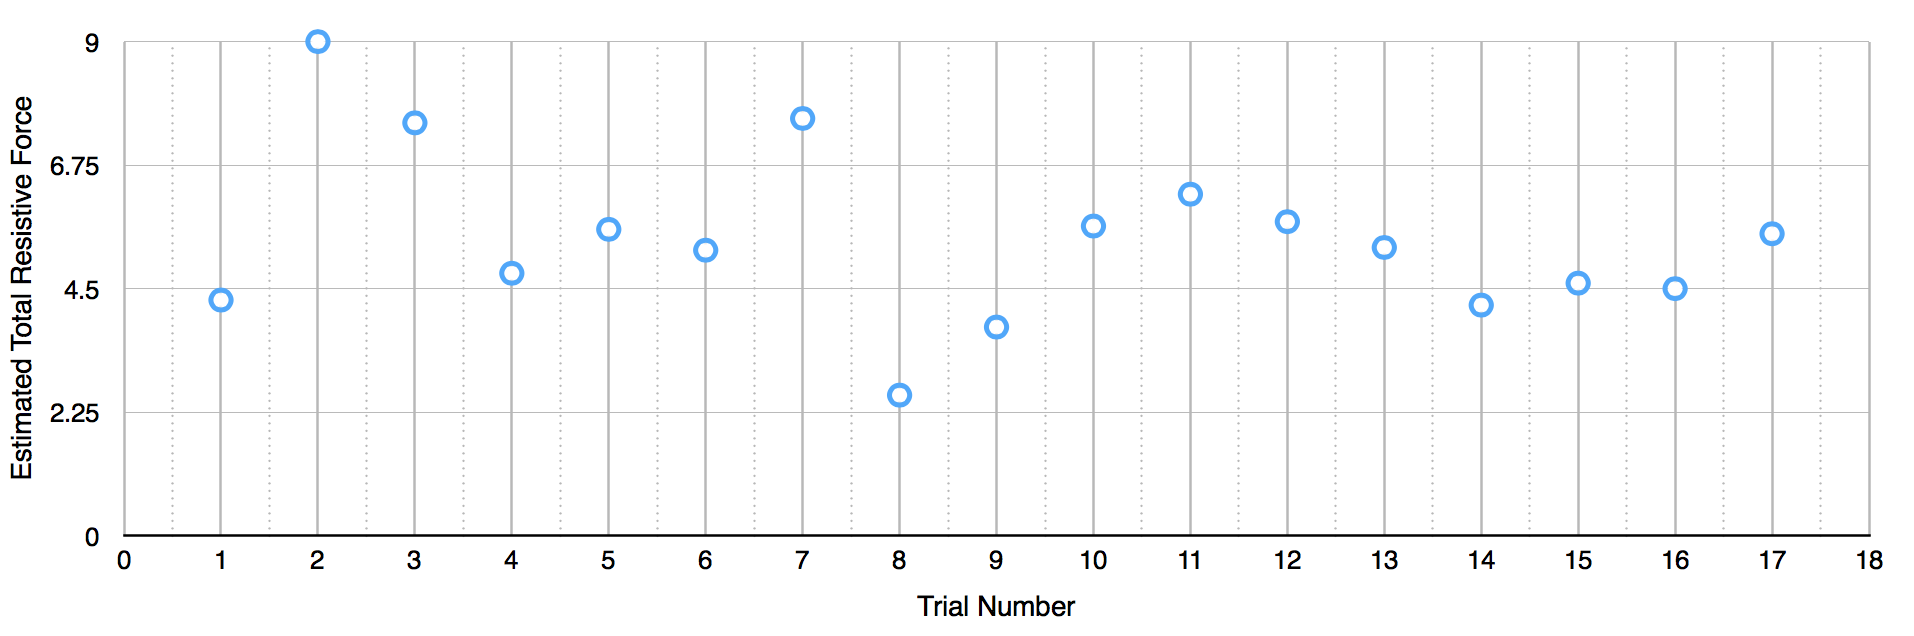
\includegraphics[width=0.5\textwidth]{figures/Ft.png}
\caption{Steady State Resistive Force Prediction Using a Normal Force Input of 4 N}
\label{fig:8}
\end{center}
\end{figure}

\section{CONCLUSIONS}
\label{sec:5}
An online adaptive estimation system used for failure detection on a telerobotic satellite servicing task monitor is proposed and experimental assessment is presented in this paper. The core of this estimator is a the recursive least squares with vector-like forgetting factors. Efforts have been made to identify situations 
when the adaptive estimator is not valid including cutter not in motion, cutter not in contact, system with low observability as well as measurements that yield unreasonable estimates (negative coefficient of friction) due to noise. Under these circumstances previous valid parameter estimates are passed into the task monitor to perform failure detection. This throttling process is important in ensuring steady performance of the estimator. We have showed through a number of experiments that the estimator is able to detect failures with an acceptable accuracy and performs consistently across different trials of the same experiment. For future work, finding an optimal set of the tunable estimator parameters (and/or a systematic way of tuning the parameters) is crucial in the improvement of the estimator's usability.

%%%%%%%%%%%%%%%%%%%%%%%%%%%%%%%%%%%%%%%%%%%%%%%%%%%%%%%%%%%%%%%%%%%%%%%%%%%%%%%%

%\section*{ACKNOWLEDGMENT}


%%%%%%%%%%%%%%%%%%%%%%%%%%%%%%%%%%%%%%%%%%%%%%%%%%%%%%%%%%%%%%%%%%%%%%%%%%%%%%%%

\label{Bibliography}


\bibliographystyle{plain} % Use the "unsrtnat" BibTeX style for formatting the Bibliography

\bibliography{icra2015} % The references (bibliography) information are stored in the file named "Bibliography.bib"


\end{document}
